\documentclass[a4paper, 11pt, titlepage]{jsarticle}
\usepackage[dvipdfmx]{graphicx}
\usepackage{amsmath}
\usepackage{listings}
\usepackage[utf8]{inputenc}
\usepackage{subfigure} % 追加
\usepackage{subcaption}
\usepackage{pgfplots}  % 追加

\title{File書き出し速度の測定}
\author{渡久山 盛正}
\date{1月20日}

\begin{document}

\maketitle

\section{実験に関する考察}

Buffered Writerは一度にまとめて書き込みを行うため、システムコールの回数が減り、効率が向上すると考えられる。ただし、バッファサイズとファイルサイズは密接に関連してと考えるため、ファイルサイズを0byteから9000byteまで、バッファサイズを0byteから32768byteまで変化させて実験を行った。考察に用いたMindMapを以下の図\ref{mind}に示す。

\begin{figure}[htbp]
	\centering
	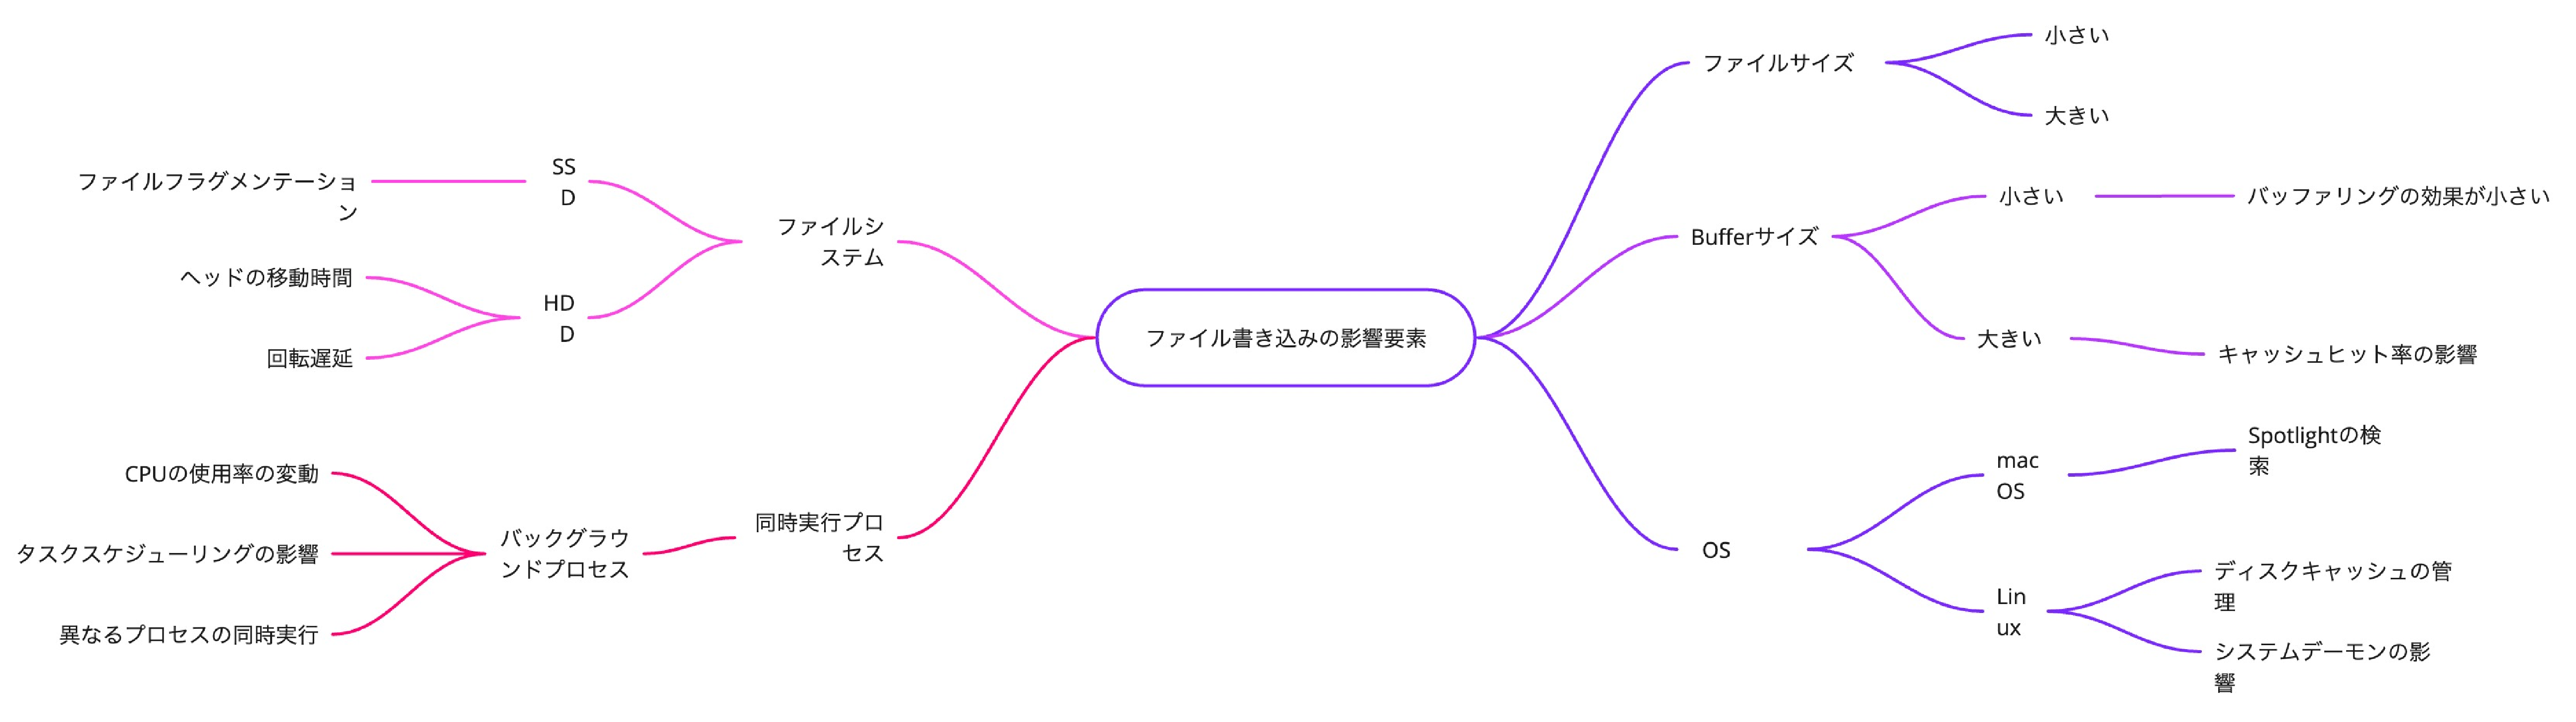
\includegraphics[width=140mm]{../img/MindMap.pdf}
	\caption{考察したMindMap}
	\label{mind}
\end{figure}

\section{実験結果}
1月19日22:15頃に実験を行った。また、ファイルサイズを0byteから9000byteまでの書き込みを行った。図\ref{filewrite1}がbuffered無しからbufferedサイズ64byteまで、図\ref{filewrite2}がbufferedサイズ64byteから32768byteまでの書き込みである。

実験結果から、bufferedがある方がファイルサイズの書き込み速度が速いことがわかった。しかし、bufferedサイズが512byteから32768byteの書き込み時間の差があまりないことから、bufferedサイズはある程度大きくなると、あまり意味がないことがわかる。

\clearpage

\begin{figure}[htbp]
  \begin{minipage}[b]{0.45\linewidth}
    \centering
    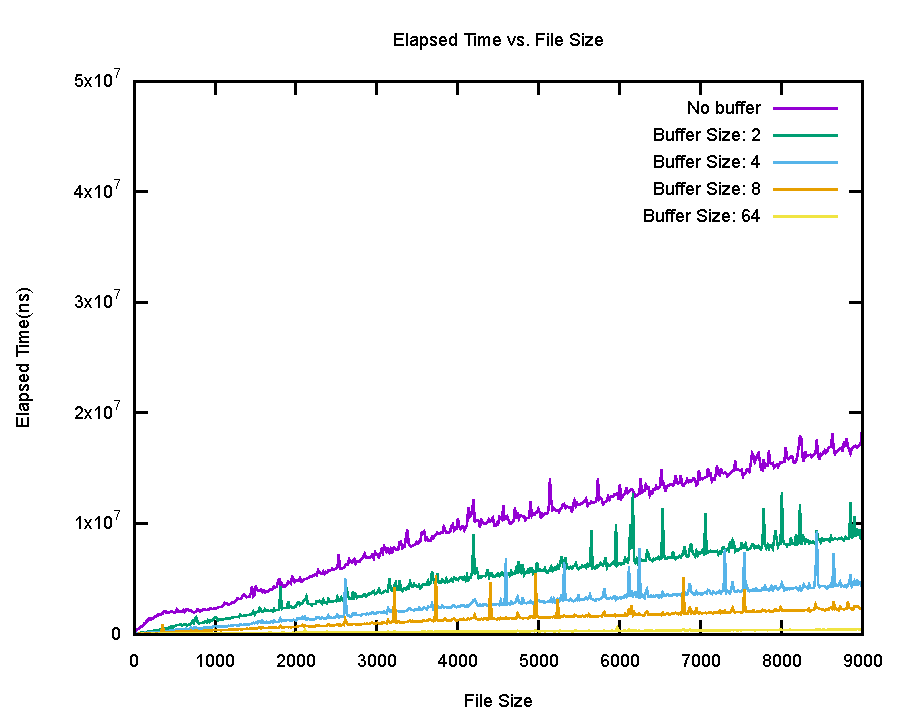
\includegraphics[keepaspectratio, scale=0.5]{../img/outputTime.pdf}
    \caption{ファイル書き込み時間}
    \label{filewrite1}
  \end{minipage}
  \hspace{0.09\linewidth}
  \begin{minipage}[b]{0.45\linewidth}
    \centering
    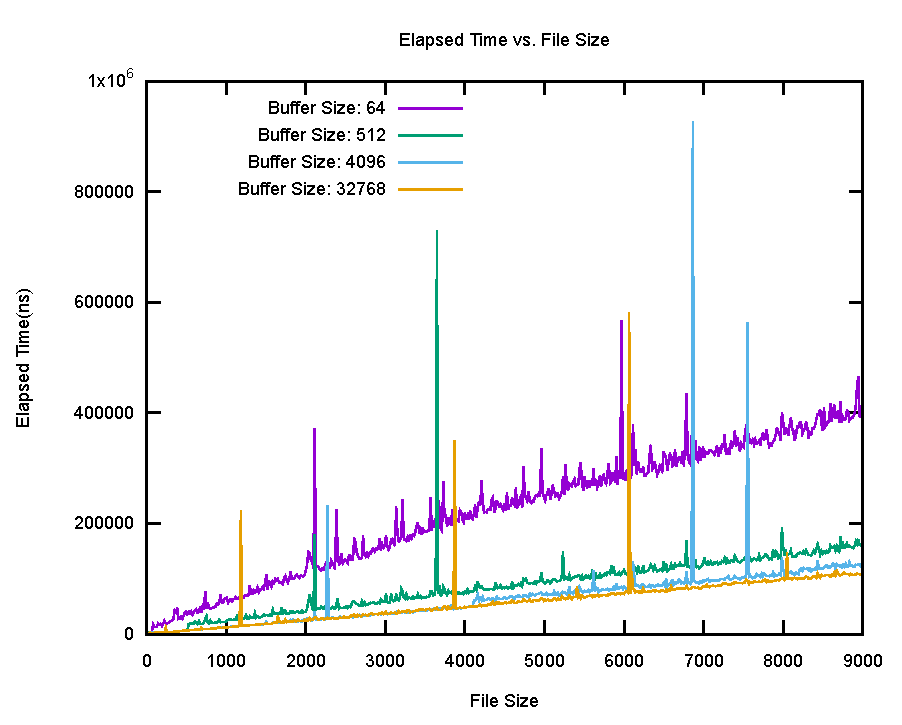
\includegraphics[keepaspectratio, scale=0.5]{../img/outputTime2.pdf}
    \caption{ファイル書き込み時間2}
    \label{filewrite2}
  \end{minipage}
\end{figure}


\section{考察}
bufferedがある方がファイル書き込み時間が速いことから、データをメモリ内で一時的に蓄積され、まとめてディスクに書き込まれる方が効率的なことがわかる。また、bufferedサイズがある程度大きくなった時に、書き込み時間にあまり変化が見られなかったのは、オーバーヘッドが大きくなることや目おりアクセス時間が増加するためだと考えられる。また、書き込み時間が直線ではなくギザギザしている原因は、CPUが他のプロセスを実行し、一時的にCPUの稼働率が減少したためだと考察する。

以上からメモリの使用量が増加することやディスクI/Oの不均衡が起こるため、bufferedサイズを最適化する必要がある。今回の実験では、512byteが最適だったと考察する。

\clearpage

\begin{thebibliography}{99}
\bibitem{class materials} golangの日記,2018-11-09,https://golang.hateblo.jp/entry/2018/11/09/163000\#ファイルの作成読み書き両方---
\bibitem{class materials2}バッファとはなに?ビジネス+全分野を網羅して日本一わかりやすく解説!,2023年12月26日,https://kyozon.net/list/what-is-buffer/
\end{thebibliography}



\end{document}
